%!TEX root = ../main.tex
\capitulo{Marco Teórico}

\seccion{Antecedentes de la Investigación}

 G. Hochmuth (2003), publicó un artículo en la Universidad de Stanford donde 
hace uso de algoritmos genéticos para desarrollar un programa que evolucione hacia 
una estrategia perfecta en el juego Tres en Línea. El autor redujo todos los posibles 
juegos a sólo 827 aprovechando la simetría del campo de juego y tomando sólo en 
cuenta las posibles jugadas que lleven por lo menos hacia un empate; aclara que este 
número de posibles jugadas fue encontrado empíricamente.  

 Este método le permitió desarrollar una estrategia perfecta después de 373 
generaciones donde el programa no perdió ni un solo juego. Se debe resaltar que el 
autor consideró como perfecta a una estrategia en la que el programa no pierde. Este 
artículo lleva por nombre On the Genetic Evolution of a Perfect Tic-Tac-Toe 
Strategy. 

 B. Blum (2002), realizó un proyecto en la Universidad de Virginia donde 
entrena a una red neuronal para jugar Tres en Línea. El autor utilizó dos redes 
neuronales: una para aprender las reglas del juego y otra para aprender una estrategia 
competente en el juego. La primera es el jugador en sí, el cual aprende a ejecutar 
jugadas legales; la segunda le indica a la primera lo que sería bueno jugar.  

 El jugador consiste en una red neuronal backpropagation con nueve neuronas 
de entrada, nueve de salida y un número variable en la capa oculta, cuando realiza 
una jugada ilegal se debilitan los pesos y cuando es legal se incrementan. La segunda 
red neuronal tiene el mismo diseño y se entrena para aprender una estrategia. Para 
entrenarlas, creó un campeonato entre 10 jugadores y elige el mejor para ser probado 
compitiendo con el humano o con otros sistemas inteligentes desarrollados también 
por el autor (uno que bloquea las jugadas ganadoras del adversario; y el otro que 
primero busca bloquear, luego ganar y si no, juega aleatoriamente). 

 Finalmente, el autor aclara que no pudo desarrollar un jugador que jugará 
perfectamente Tres en Línea pero logró que realizaran un 100\% de jugadas legales. 
Este proyecto tiene por nombre Neural Net Training for Tic Tac Toe. 

 La empresa ADIT Software desarrolló un software inteligente para jugar Tres 
en Línea, donde utiliza 200 redes neuronales con nueve neuronas de entrada, nueve 
de salida y diez ocultas. Cada una realizó 100 juegos (con otra asignada 
automáticamente) de los cuales en 50 comenzaba. Luego, utilizó algoritmos genéticos 
para escoger la mejor. Según la empresa: este sistema era fuerte atacando pero a 
veces fallaba defendiendo; ganaba un número razonable de veces pero también perdía 
mucho incluso después de 1000 generaciones. Este software se llama MENACE y el 
sistema siempre juega de primero. No especifica fecha de creación. 
 
 En 1999 se desarrolló un robot para jugar Tres en Línea, el cual fue llevado al 
festival MindFest de inteligencia artificial que se desarrolló en el Instituto 
Tecnológico de Massachussets (MIT) de Estados Unidos en el mismo año. Este 
proyecto fue realizado por M. Beri, G. Ferrari y M. Ferrari, y consiste en un robot 
construido con materiales de Lego® Mindstorms. El robot coloca la pieza 
correspondiente a su jugada en el campo de juego, detecta cuando es su turno además 
sí hay ganador o no. Aunque el robot no puede aprender, este realiza su jugada 
basándose en algunas estrategias limitadas cuyos autores decidieron no publicar. El 
proyecto responde al nombre de A Lego®Mindstorms Tic-Tac-Toe Player. 


\seccion{Bases Teóricas}

	\seccion{Mecánica}
	
		\subseccion{Leyes de Newton}
		En la segunda mitad del siglo XVII, Sir Isaac Newton formuló tres leyes 
		fundamentales en las que se basa la ciencia mecánica. Estas son enunciadas por F. 
		Beer et al (1990) como sigue: 
		\begin{enumeracion}
		\item PRIMERA LEY. Si la fuerza resultante que actúa sobre una partícula es cero, la 
		partícula permanecerá en reposo (si originalmente estaba en reposo) o se moverá 
		con velocidad constante en una línea recta (si originalmente estaba en 
		movimiento. 
		\item SEGUNDA LEY. Si la fuerza resultante que actúa sobre una partícula no es cero, 
		la partícula tendrá una aceleración proporcional a la magnitud resultante y en la 
		dirección de ésta. 
		\item TERCERA LEY. Las fuerzas de acción y reacción de cuerpos en contacto tienen 
		la misma magnitud, la misma línea de acción y sentidos opuestos. 
		\end{enumeracion}
	
	\subseccion{Equilibrio}
	
		 Se dice que un cuerpo está en equilibrio cuando la resultante de las cargas 
		externas y reacciones que actúan sobre el cuerpo es igual a cero; esto es, la suma de 
		todas las fuerzas (o de sus componentes) actuando en cualquier dirección posible 
		debe ser igual a cero. Además, también debe ser cero la suma de los momentos de 
		todas las fuerzas respecto a cualquier eje. 
		
		 Para que una estructura o parte de ella esté en equilibrio bajo la acción de un 
		sistema de cargas, debe satisfacer las seis ecuaciones de equilibrio de la Estática. 
		Utilizando los ejes cartesianos x, y y z, las ecuaciones pueden escribirse como sigue
		
		\begin{ecuacion}{}
			\sum{F_{x} = 0}; \sum{F_{y} = 0}; \sum{F_{z} = 0};
			% \sum{M_{x} = 0}; \sum{M_{y} = 0}; \sum{M_{z} = 0}
		\end{ecuacion}		
		
		 Estas ecuaciones no pueden demostrarse algebraicamente; sólo describen la 
		afirmación de Sir Isaac Newton: para cada acción sobre un cuerpo en reposo, hay una 
		reacción igual y opuesta. 

		 Una estructura puede encontrarse en equilibrio estable o inestable. Según J. 
		Kinney (1981), una estructura en equilibrio estable indica que ésta podrá soportar 
		cualquier sistema concebible de cargas aplicadas. Es importante destacar que aunque 
		una estructura sea estable para soportar uno o varios conjuntos de cargas, si no es 
		estable para cualquier conjunto de cargas entonces se dice que se encuentra en 
		equilibrio inestable. Frecuentemente, una estructura en equilibrio inestable será 
		estable bajo un sistema particular de cargas aplicadas. 

		\subseccion{Modelo y análisis matemático para el diseño estructural del brazo}
		
		Según J. Kinney (1981), \textquotedblleft una estructura articulada está compuesta de 
		eslabones o barras, que se suponen conectadas por pasadores carentes de fricción en 
		las juntas\textquotedblright. Con esta descripción, es claro que un brazo mecánico es una estructura 
		articulada. El modelo matemático del brazo articulado se describe en la figura uno.
		
		 Se puede notar que: el pasador a permite la rotación de la estructura en el eje 
		y; el pasador b permite desplazamientos de la estructura perpendiculares al eje z; y, 
		el pasador c permite girar el eslabón B perpendicularmente al eje z. 
		
		\begin{ecuacion}{}
			\sum{F_{x} = 0};\sum{F_{y} = 0};\sum{F_{z}=0};
		\end{ecuacion}
		
		 En la figura 1, a pesar de que el punto h se desplaza en tres dimensiones, los 
		eslabones A y B realizan sus desplazamientos en un plano cualquiera denotado por 
		yx. Asimismo, las cargas que actúan sobre la estructura son pesos cuyas líneas de 
		acción también se encuentran en el plano yx. 
		
		\begin{ilustracion}
			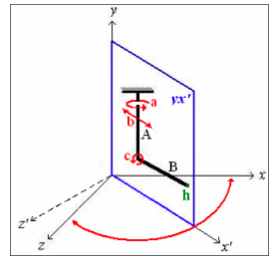
\includegraphics{figures/figura-1.png}
			\tituloilustracion{Modelo Matemático del Brazo Mecánico}{et:modelobrazo}
		\end{ilustracion}
		
		 Dado que las cargas, eslabones y desplazamientos relativos, se encuentran en 
		el mismo plano (cargas coplanares), es posible analizar la estructura en dos 
		dimensiones. En este caso, J. McCormac et al. (1994) establece que 
		
	\citatextual{
			la suma de las 
		fuerzas en las direcciones x y y, así como la suma de los momentos respecto a un eje 
		perpendicular al plano debe ser cero. Definiendo así las siguientes ecuaciones de 
		equilibrio para esta estructura 
}
		
		\begin{ecuacion}{}
			\sum{F_{x} = 0}; \sum{F_{y} = 0}; \sum{M_{z} = 0}
		\end{ecuacion}
		
		 El brazo mecánico es una estructura en equilibrio inestable, y utilizando 
		motores eléctricos paso a paso se logra anular la fuerza de inercia. Para lograr que la 
		estructura se desplace como indica el modelo matemático (figura 1), se puede utilizar 
		la siguiente configuración 
		
		\begin{ilustracion}
			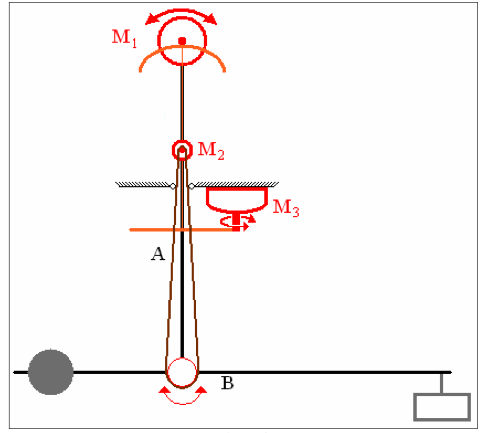
\includegraphics{figures/figura-2.png}
			\tituloilustracion{Brazo Mecánico con Motores Paso a Paso}{et:motorespaso}
		\end{ilustracion}
		
		 Esta estructura se puede descomponer y así analizar cada eslabón por 
		separado, esto es porque tanto el eslabón A como el B son cuerpos en equilibrio. Así, 
		el diagrama de cuerpo libre para el eslabón B es 
		
		\begin{ilustracion}
			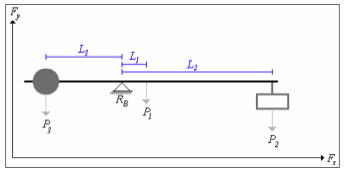
\includegraphics{figures/figura-3.png}
			\tituloilustracion{Diagrama de Cuerpo Libre – Eslabón B}{et:dcl-B}
		\end{ilustracion}
		
		donde P1 es el peso del eslabón aplicado en su centro de gravedad, 
		 $L_{1}$ es la distancia de $P_{1}$ al punto de apoyo $R_{B}$, 
		 $P_{2}$ es el peso de la carga, 
		 $L_{2}$ es la distancia de $P_{2}$ al punto de apoyo $R_{B}$,
		 $P_{3}$ es el peso de la contrapesa, y 
		 $L_{3}$  es la distancia de $P_{3}$ al punto de apoyo $R_{B}$.
		
		Para que el cuerpo se encuentre en equilibrio se debe cumplir que 
		
		\begin{ecuacion}{}
			\sum{F_{y}}:P_{1}+P_{2}+P_{3}-R_{B} = 0
		\end{ecuacion}
		\begin{ecuacion}{}
			\sum{M_{R_{B}}}:P_{1}\times L_{1}+P_{2}\times L_{2}-P_{3}\times L_{3} = 0
		\end{ecuacion}
		
		Ahora, el diagrama de cuerpo libre para el eslabón A es como sigue: 
	 
		\begin{ilustracion}
			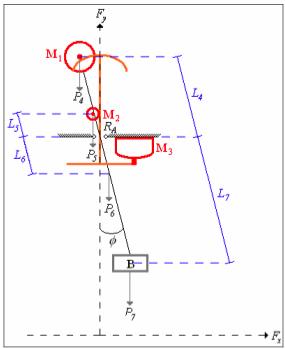
\includegraphics{figures/figura-4.png}
			\tituloilustracion{Diagrama de Cuerpo Libre – Eslabón A}{et:dcl-a}
		\end{ilustracion}
		
		donde $P_{4}$ es el peso del motor $M_{1}$, 
		 $L_{4}$ es la distancia de $P_{4}$ al punto de apoyo $R_{A}$, 
		 $P_{5}$ es el peso del motor $M_{2}$, 
		 $L_{5}$ es la distancia de $P_{5}$ al punto de apoyo $R_{A}$, 
		 $P_{6}$ es el peso del eslabón $A$ aplicado en su centro de gravedad,  
		 $L_{6}$ es la distancia de $P_{6}$ al punto de apoyo $R_{A}$. 
		 $P_{7}$ es el peso del eslabón $B$, y  
		 $L_{7}$ es la distancia de $P_{7}$ al punto de apoyo $R_{A}$. 
		
		 Para que este cuerpo esté en equilibrio se debe cumplir entonces que 
		\begin{ecuacion}{}
				\sum{F_{y}}:P_{4}+P_{5}+P_{6}+P_{7}-R_{A}=0
		\end{ecuacion}
		\begin{ecuacion}{}
			\sum{M_{R_{A}}}:-P_{4}\times\left(L_{4}\sin\theta\right) -P_{5}\times\left(L_{5}\sin\theta\right) +P_{6}\times\left(L_{6}\sin\theta\right) +P_{7}\times\left(L_{7}\sin\theta\right) = 0
		\end{ecuacion}
		
		 Observando la ecuación de momento en el punto de apoyo RA, se observa que 
		$\sin\theta$ es común en todos los elementos. Esto significa que el cuerpo se encontrará en 
		equilibrio para cualquier ángulo. 
		
		Ya establecidas las ecuaciones de equilibrio para esta estructura, el diseño 
		puede ser llevado a cabo. 
		
		\subseccion{Engranajes}
			Los engranajes son utilizados para transmitir potencia de un eje a otro. Véase 
		la siguiente figura.
		
		\begin{ilustracion}
			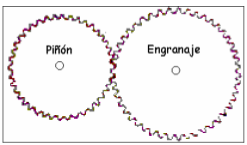
\includegraphics{figures/figura-5.png}
			\tituloilustracion{Piñón – Engranaje}{et:engranaje}
		\end{ilustracion}
		
		 La relación de engranajes viene dada por $n=N_{P}/N_{E}$ donde $N_{P}$ es el número de 
		dientes del piñón y $N_{E}$ es el número de dientes del engranaje. 

		 La velocidad de salida (Engranaje) respecto a la de entrada (Piñón) está 
		determinada por $\omega_{E}=n\omega_{p}$.
		 Y, el par motor de salida es determinado por $T_{E}=T_{P}/n$.
	
	\seccion{Electrónica}	
	Antes de explicar lo referente al microcontrolador 8951 es necesario aclarar 
	que no se trata de un manual para su uso, se trata de la teoría en que se basó este 
	trabajo de grado incluyendo algunos detalles importantes basados en previas 
	experiencias del autor. 
	
	\subseccion{Microcontrolador 8951} 
	 El microcontrolador 8951 pertenece a la familia de microcontroladores MCS- 
	51. Según M. Martos et al., esta familia consiste en cuatro miembros compatibles pin 
	a pin que son el 8031, 8051, 8751 y 8951; los cuales se diferencian en la memoria de 
	programa ROM. 
	
	 Según A. Vega (1999), el microcontrolador 8951 tiene las siguientes 
	características: CPU de 8 bits como parte central, 32 líneas bidireccionales de entrada 
	y salida (4 puertos), 128 bytes de memoria RAM, 2 Contadores / Temporizadores de 
	16 bits, 5 estructuras de interrupción con dos niveles de prioridad, 64 KBytes de 
	espacio para programa y 64 Kbytes de espacio para datos. La estructura física se 
	observa a continuación. 
	
	\begin{ilustracion}
		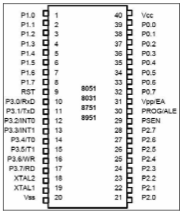
\includegraphics{figures/figura-6.png}
		\tituloilustracion{Microcontrolador MCS-51}{et:micro}
	\end{ilustracion}
	
	\subsubseccion{Puerto P0}
	 Este puerto se puede utilizar para convertirlo en bus de datos o direcciones 
	cuando el pin EA es conectado a 0v (0 lógico), este se encarga de la parte baja del bus 
	cuando se utiliza memoria externa. Es importante señalar que este puerto no es 
	adecuado para emitir señales de 5v (1 lógico) ya que las salidas del mismo están en 
	alta impedancia. 
	
	\subsubseccion{Puerto P1}
	 Es un puerto bidireccional de 8 bits cuya etapa de salida puede manejar 
	corrientes equivalentes a cuatro cargas TTL LS. Este puerto no tiene funciones 
	secundarias. 
	
	\subsubseccion{Puerto P2} 
	 Al igual que el puerto P1, es un puerto bidireccional de 8 bits y puede manejar 
	corrientes equivalentes a cuatro cargas TTL LS. Este puerto tiene como función 
	secundaria la de suministrar la parte alta de la dirección cuando es necesario recurrir a 
	memoria externa. 
	
	\subsubseccion{Puerto P3} 
	 Igual que los puertos anteriores, pero la función secundaria de los pines son: 
	P3.0/RxD, entrada para la comunicación serial; P3.1/TxD, salida para la 
	comunicación serial; P3.2/INT0, entrada para la interrupción externa 0; P3.3/INT1, 
	entrada para la interrupción externa 1; P3.4/T0 y P3.5/T1, entradas respectivas de 
	conteo para los Timer 0 y 1; P3.6/WR y P3.7/RD, salidas respectivas que indican la 
	escritura o lectura de la memoria externa. 
	
	Los pines pueden ser configurados independientemente, es decir, si no se 
	utilizarán las funciones secundarias de algunos pines, estos pueden ser utilizados 
	libremente por el programador para otros fines. 
	
	\subsubseccion{Otros pines} 
	 Los pines Vcc y Vss son para la alimentación del microcontrolador, deben 
	conectarse respectivamente a +5v y a 0v. Los pines correspondientes a XTAL1 y 
	XTAL2 son para conectar el cristal oscilador que determinará la frecuencia con que 
	funcionará el reloj del microcontrolador, generalmente se emplean cristales 
	osciladores de 11.059 MHz o 12 MHz. Es importante tomar en cuenta la frecuencia 
	de oscilación tanto para las rutinas de retardo como para la comunicación serial y 
	temporizadores, ya que los ciclos de máquina dependen de esta frecuencia. 
	
	 El pin RST sirve para reiniciar el microcontrolador cuando se le envía una 
	señal alta (1 lógico) durante dos ciclos de máquina, el proceso de reinicio causa una 
	interrupción en la dirección 00h. 
	
	 El pin Vpp/EA sirve para acceder a memoria externa. Cuando se utiliza 
	memoria externa para almacenar las instrucciones a ejecutar por el microcontrolador, 
	se debe conectar a 0 lógico. Cuando esto ocurre, los puertos P0 y P2 desempeñan las 
	funciones secundarias. Ahora, en caso de que las instrucciones hayan sido 
	almacenadas en la memoria interna del microcontrolador, deberá conectarse a 1 
	lógico. 
	
	 El pin PROG/ALE fija el byte bajo de la dirección durante el acceso a 
	memoria externa y, cuando no se utiliza memoria externa, emite un rango constante 
	de 1/6 de la frecuencia del oscilador que, según A. Vega (1999), puede ser utilizado 
	para cronometrar. 
	
	 Finalmente, el pin PSEN habilita la lectura para memoria de programas 
	externos. 
	
	\subsubseccion{Memoria RAM Interna}
	El microcontrolador 8951 posee cuatro bancos de ocho registros cada uno, 
	donde cada registro está conformado por 8 bits. También posee 16 bytes de memoria 
	que son direccionable bit a bit lo cual permite utilizar banderas adicionales, y 80 
	bytes más para uso general.  
	
	 La memoria del microcontrolador 8951 se segmenta de la siguiente manera 
	Registros: desde la dirección 00h hasta la dirección 07h se ubican los registros R0 a 
	R7 del banco 0; de 08h a 0Fh, los registros R0 a R7 del banco 1; de 10h a 17h los 
	registros R0 a R7 del banco 2; y de 18h a 1Fh los registros del banco 3. Suman un 
	total de 32 bytes destinados a registros. A todos se pueden acceder pero es necesario 
	modificar los bits RS0 y RS1 del registro PSW; por defecto los valores son 0 y 0, lo 
	cuál indica que se está trabajando en el banco 0. Para trabajar con el banco 1 se debe 
	establecer RS0=0 y RS1=1; para el banco 2, RS0=1 y RS1=0; y para el banco 3, 
	RS0=1 y RS1=1. 
	
	Direccionable bit a bit: desde la dirección 20h hasta la dirección 2Fh son celdas a las 
	que se puede acceder bit a bit (e.g. 20h.0, 2Fh.7); la cantidad total es de 16 bytes. 

	Memoria de uso general: desde la dirección 30h hasta la dirección 7Fh, lo cual suma 
	80 bytes para uso general. 

	 El área de memoria a partir de la dirección 80h hasta la dirección FFh, 
	pertenece los registros de interrupciones, configuración de los temporizadores, 
	acumulador, etc. 
	
	\subsubseccion{Comunicación Serial}
	 La comunicación serial se implementa utilizando cualquiera de los 
	temporizadores para generar la velocidad de transmisión/recepción de datos. Tanto 
	para enviar como para recibir datos se debe hacer uso del registro SBUF. Este registro 
	almacena 1 byte que será recibido o transmitido. Un aspecto importante, es que tanto 
	el microcontrolador como el PC deben ser configurados a la misma velocidad de 
	transmisión/recepción. 
	
	 Un computador personal permite conexiones, a través del puerto serial, a las 
	siguientes velocidades: 110, 300, 1200, 2400, 4800, 9600, 19200, 38400, 57600, 
	115200 bps, utilizando Microsoft HyperTerminal; por lo que al momento de 
	configurar la velocidad de transmisión/recepción en el microcontrolador, se debe 
	aplicar la siguiente fórmula (A. Vega (1999)) 
	
	\begin{ecuacion}{}
		BaudRate={2^{SMOD}\times Freq}/{32\times\left(256-THx\right)}
	\end{ecuacion}
	
	donde Baud Rate es la velocidad en bps; Freq es la frecuencia de oscilación 
	(determinada por el cristal); SMOD determina el divisor de frecuencia (0 para 1/32 ó 
	1 para 1/64); y THx, es el valor de recarga para el temporizador 0 ó 1. 
	 Para aplicar la fórmula: se conoce la velocidad de transmisión/recepción de 
	datos (e.g. 9600 bps), se conoce la frecuencia de oscilación (e.g. 11.059 MHz) y el bit 
	SMOD es determinado a nivel de programación (e.g. 0). Para este caso, es necesario 
	despejar la variable THx a fin de determinar la velocidad de transmisión/recepción de 
	datos. 
	
	 Es importante señalar que el resultado de THx debe ser aproximado a un 
	entero menor que 256 debido que para asignar el valor de recarga es necesario un 
	entero no mayor a 8 bits (capacidad de THx). En caso de usar del temporizador 1 en 
	modo 2 y para las especificaciones expuestas en el párrafo anterior, al despejar THx 
	el resultado es 253.00005. Esto indica que para lograr configurar la comunicación 
	serial a una velocidad de transmisión/recepción de 9600 bps, utilizando un cristal 
	oscilador de 11.059 MHz y SMOD = 0, el valor con que debe ser cargado TH1 es 
	FDh (253 en decimal). 
	
	 La comunicación serial, con las especificaciones expuestas, funciona sin 
	contratiempos. Esto se debe a que 253.00005 es muy aproximado a 253, el problema 
	que puede surgir es al momento de utilizar una velocidad distinta a 9600 bps o al 
	utilizar un cristal oscilador con una frecuencia distinta a 11.059 MHz. Para esto, es 
	necesario volver a aplicar la fórmula con las nuevas especificaciones y, en caso de 
	obtener un valor (THx) no muy aproximado a un entero (e.g. 253.5) se debe probar 
	con diferentes configuraciones, ya que este valor es determinante para lograr la 
	velocidad de transmisión/recepción. 
	
	 Otro ejemplo, si se desea trabajar con un cristal oscilador de 12 MHz es 
	necesario bien modificar el modo de operación del temporizador o la velocidad de 
	transmisión/recepción, ya que el valor obtenido para TH1 (en caso de utilizar el 
	temporizador 1) no es muy exacto. Esto se puede resolver utilizando una velocidad de 
	1200 bps, SMOD = 0, temporizador 1 en modo 2; ya que al momento de aplicar la 
	fórmula, el valor de TH1 es 229.95 $\approx$ 230 (E6 en hexadecimal). 
	
	 Por último, pero no menos importante, para la comunicación serial con una 
	computadora es necesario utilizar el circuito integrado MAX232 (en caso de usar la 
	norma RS-232) ya que los niveles lógicos del microcontrolador son TTL y la 
	computadora utiliza 0 = -12v y 1 = 12v. Este circuito integrado funciona como 
	interfaz: cuando recibe datos del PC estos son convertidos a los niveles lógicos del 
	microcontrolador y, cuando se envían datos desde el 8951, estos son convertidos a 
	niveles lógicos del computador.  

	\subseccion{Otros Componentes}
		\subsubseccion{Latch} 
	 Los latch son utilizados para funcionar como memoria externa volátil, aunque 
	permiten almacenar poca información (el 74LS175 almacena 4 bits y sus negados) 
	estos pueden ser utilizados para expandir los puertos del microcontrolador. 
	Particularmente, el 74LS175 consta de cuatro entradas, ocho salidas (las cuatro 
	entradas y sus negados), un pin para limpiar la memoria (CLR) y otro para determinar 
	cuando el latch debe almacenar la información. 
	
	 El diagrama del latch 74LS175 se puede observar a continuación 
	
	\begin{ilustracion}
		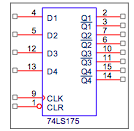
\includegraphics{figures/figura-7.png}
		\tituloilustracion{Diagrama – 74LS175}{et:latch}
	\end{ilustracion}
	
	\subsubseccion{Motores Paso a Paso}
	 La característica más importante de los motores paso a paso es que permiten 
	un movimiento controlado, lo cual permite ajustar la velocidad a fin de evitar fuerzas 
	de inercia. Entre otras características se puede mencionar que son precisos, fuertes y 
	de fácil control (respecto a los servomotores). 
	
	 Los motores paso a paso pueden ser bipolares o unipolares. Los bipolares 
	requieren el uso de un puente H para su manejo, ya que funcionan con voltajes 
	positivos y voltajes negativos (e.g. +12v, -12v). Los unipolares no necesitan de 
	puente H, ya que trabajan con voltaje positivo y tierra (e.g. +5v y 0v). Estos dos tipos 
	de motores pueden diferenciarse físicamente por la cantidad de cables: los bipolares 
	poseen cuatro cables y los unipolares poseen cinco o seis cables. 
	
	 En este trabajo de grado es de interés los motores unipolares, por lo cual se 
	explican a continuación. 
	
	 Los motores unipolares funcionan mediante la activación de bobinas, las 
	cuales al ser activadas generan un campo magnético que permiten hacer girar al piñón 
	cierto ángulo. Este ángulo viene determinado por el fabricante del motor. 
	
	 Para hacer girar a un motor paso a paso, es necesario conseguir la secuencia 
	de activación y desactivación de bobinas; pero primero se debe conocer cual es el 
	punto común de las bobinas (cuando el motor tiene 5 cables, tiene un solo punto 
	común; cuando son 6 cables tiene dos puntos comunes, uno para cada par de 
	bobinas).  
	
	 El punto común se consigue midiendo la resistencia ($\Omega$) entre cada uno de los 
	cables respecto a los demás; cuando en un cable la resistencia es igual respecto a 
	cualquier otro cable, significa que es un punto común. El valor de esta resistencia 
	también lo especifica el fabricante. 

	 Una vez localizado el (los) punto(s) común(es), se puede controlar el motor de 
	dos maneras: a) conectando el punto común al voltaje que especifica el motor, o b) 
	conectando el punto común a tierra (0v). En la primera, la activación de bobinas se 
	debe realizar conectando el cable de la bobina respectiva a tierra (0v). En la segunda, 
	es necesario conectarlo al voltaje indicado por el fabricante. 
	
	 Ya establecida la conexión al punto común, el movimiento del motor se puede 
	realizar de tres formas distintas:
	\begin{enumeracionenparrafo}
		\item bobina en bobina, 
		\item de dos bobinas en dos bobinas, o 
		\item utilizando medio paso (Half Stepping).
		\end{enumeracionenparrafo}
		
	Las secuencias de activación se reflejan en el cuadro 1. 
	
	 El cuadro \ref{cuadro:1} describe la secuencia de activación de bobinas para hacer girar el 
	motor en una dirección. En cuanto a estas formas se puede decir que:
	\begin{enumeracionenparrafo}
		\item la forma de 
	bobina en bobina no es muy usada, ya que de esta forma el motor tiene menos torque 
	que utilizándolo de dos en dos bobinas, 
	\item de dos en dos bobinas permite dar pasos en 
	el ángulo que especifica el fabricante y con más torque que la forma anterior,
	\item 
	utilizando medio paso, cada paso que da el motor es la mitad del ángulo que 
	especifica el fabricante. 
	\end{enumeracionenparrafo}
	
	 Es importante destacar que para el uso de motores paso a paso con el 
	microcontrolador, no se deben conectar los cables del motor directamente a los pines 
	ya que los requisitos de corriente para los motores paso a paso generalmente es 
	elevado (alrededor 1 Amp). Para su uso se recomienda utilizar transistores (e.g. TIP- 
	122).
	
	\begin{cuadro}{l rrrr}{Secuencias Paso a Paso}{cuadro:1}
		\toprule
		Bobino&\multicolumn{4}{c}{Bobina por bobina}\\
		\midrule
		on&Bobina A& Bobina B & Bobina C & Bobina D\\
	   on& On &Off &Off& Off \\
	   on& Off &On &Off &Off \\
	   on& Off &Off& On &Off\\
	   on& Off &Off& Off &On\\
		% \midrule
		% \multicolumn{4}{c}{De dos en dos bobinas} \\ 
		% \midrule
		% On &On &Off& Off \\
		% Off& On &On &Off \\
		% Off &Off& On &On \\
		% On &Off& Off &On \\
		% \midrule
		% \multicolumn{4}{c}{Medio Paso (Half Stepping)} \\
		% \midrule
		% On &Off& Off& Off\\
		% On &On &Off &Off \\
		% Off& On& Off& Off\\
		% Off& On& On &Off \\
		% Off& Off& On &Off\\
		% Off& Off& On &On \\
		% Off& Off& Off& On\\
		% On &Off &Off &On \\
		\bottomrule
		\fuentecuadro{5}{\yo}
	\end{cuadro}
	
	
	\begin{cuadro}{l rrrrrrr}{Título del cuadro}{titulo-cuadro-x}
		\toprule
		Audio Name&\multicolumn{7}{c}{Sum of Extracted Bits} \\ [0.5ex]    
		\midrule
		Police   & 5 & -1 &  5& 5& -7& -5& 3\\  % Entering row contents 
		Midnight & 7 & -3 &  5& 3& -1& -3& 5\\ 
		News     & 9 & -3 &  7& 9& -5& -1& 9\\[1ex] % [1ex] adds vertical space 
		\bottomrule
		\fuentecuadro{8}{\yo}

	\end{cuadro}

	
	
	
	\seccion{Teoría de Juegos}
		 El objetivo de la teoría de juegos es analizar el comportamiento estratégico de 
		los jugadores. Según R. Fischer (2000), \textquotedblleft La teoría de juegos examina el 
		comportamiento estratégico de jugadores que interactúan motivados por la 
		maximización de la utilidad y que saben que los otros participantes son racionales\textquotedblright. 
		
		 Varoufakis (2001) define la teoría de juegos como\par
		
		\citatextual{El análisis del 
		comportamiento racional bajo circunstancias de interdependencia estratégica, cuando 
		la mejor estrategia de un individuo depende de lo que sus oponentes probablemente 
		hagan. 
		comportamiento racional bajo circunstancias de interdependencia estratégica, cuando 
		la mejor estrategia de un individuo depende de lo que sus oponentes probablemente 
		hagan.comportamiento racional bajo circunstancias de interdependencia estratégica, cuando 
		la mejor estrategia de un individuo depende de lo que sus oponentes probablemente 
		hagan.comportamiento racional bajo circunstancias de interdependencia estratégica, cuando 
		la mejor estrategia de un individuo depende de lo que sus oponentes probablemente 
		hagan.comportamiento racional bajo circunstancias de interdependencia estratégica, cuando 
		la mejor estrategia de un individuo depende de lo que sus oponentes probablemente 
		hagan.comportamiento racional bajo circunstancias de interdependencia estratégica, cuando 
		la mejor estrategia de un individuo depende de lo que sus oponentes probablemente 
		hagan.
}
		
		En la teoría de juegos siempre se habla sobre lo inteligente y lo racional que 
		es un jugador. Según B. Slantchev (2004) un jugador racional es aquel que, 
		coherentemente, toma decisiones en búsqueda de un objetivo bien definido; y un 
		jugador inteligente es aquel que, sabiendo lo que los demás jugadores saben, puede 
		hacer las mismas inferencias que ellos pueden hacer. 
		
		
		De las definiciones anteriores se puede inferir que: 
		\begin{enumeracion}
		\item La teoría de juegos analiza el comportamiento estratégico de los jugadores ante 
		los posibles eventos que ocurren en el juego. 
		\item  El comportamiento racional de cada jugador viene dado por la búsqueda de 
		maximizar su utilidad. 
		\item  El comportamiento inteligente de cada jugador está determinado por la capacidad 
		de inferir la calidad de una estrategia teniendo en cuenta que los demás jugadores 
		tienen la misma capacidad. 
		\item  Un jugador racional e inteligente jugará basándose en la maximización de su 
		utilidad tomando en cuenta las jugadas que pueden hacer los demás jugadores 
		para maximizar sus respectivas utilidades. 
		\end{enumeracion}
		
		La representación de un juego en forma normal viene dada por una matriz de 
		pagos que contiene las utilidades que generará cada combinación de estrategias por 
		cada uno de los jugadores. Por ejemplo, el juego piedra, papel ó tijeras es un juego 
		de suma cero en el que dos jugadores eligen un objeto (Piedra, Papel ó Tijeras) y las 
		reglas son: Piedra le gana a Tijeras, Tijeras le ganan a Papel, Papel le gana a Piedra y, 
		si ambos eligen el mismo objeto entonces es un empate; su representación en forma 
		normal se muestra en el siguiente cuadro. \par

		
		\begin{cuadro}{cccc}{Titulo del cuadro}{otro-cuadro-mas}
			\toprule
			Jugares I y II& Piedra & Papel & Tijeras\\
			\midrule
			Piedra   & (0,0) & (-1,1) & (1,-1)\\
			Papel   & (1,-1) & (0,0) & (-1,1)\\
			Tijeras   & (-1,1) & (1,-1) & (0,0)\\
			\bottomrule
			\fuentecuadro{4}{\yo}
		\end{cuadro}
		
		 Como se puede observar en el cuadro 2, la forma normal muestra sólo los 
		resultados representados en términos de la función utilidad de cada jugador (I, II) que 
		se generan para cada combinación de estrategias. La función de utilidad (1,-1) indica 
		que gana el jugador I y pierde el jugador II, (-1,1) gana II y pierde I, y (0,0) implica 
		que I y II empatan. Es de notar que, dada cualquier combinación de estrategias, si se 
		suma la utilidad de A con la utilidad de B, el resultado siempre es cero. Esto indica 
		que Piedra, Papel ó Tijeras es un juego de suma cero. 
		

\seccion{Bases Legales}

Es completamente ilegal. Esto es un ejemplo de definición: \gls{algoritmo-evolutivo}. Esto es un ejemplo de plural \glspl{algoritmo-evolutivo}.
\begin{grafico}
	
\includegraphics[height=1in,width=1in]{figures/Miguelito.jpg}
	\titulografico{Esto debería ser un gráfico (e.g. barras)}{et:grafico}
\end{grafico}


% \seccion{Definición de Términos Básicos}
\hacerglosario % Ejecutar desde la consola "makeglossaries main" para que aparezca.



\begin{grafico}
	
\includegraphics[height=1in,width=1in]{figures/Miguelito.jpg}
	\titulografico{Esto debería ser un gráfico (e.g. de líneas)}{et:grafico1}
\end{grafico}

\seccion{Sistema de Hipótesis}

Existe la hipertesis que \LaTeX será la raíz de los próximos sistemas operativos.
% \begin{grafico}
% 	
\includegraphics[height=1in,width=1in]{figures/Miguelito.jpg}
% 	\titulografico{Esto debería ser un gráfico (e.g. tarta)}
% \end{grafico}

\seccion{Operacionalización de las Variables}

Operar variables.